\documentclass[10pt]{scrartcl}
\usepackage{graphicx}
\usepackage{float}
\usepackage{amsmath}
\usepackage[utf8]{inputenc} 
\usepackage[T1]{fontenc}
\usepackage{lmodern}
\usepackage{amsfonts}   
\usepackage{amssymb}
\usepackage{mathtools}
\usepackage{epstopdf}
\usepackage[shadow]{todonotes}

 
\begin{document}

\title{Dokumentation zum Java Code Camp 21.02.2020}

%Bitte hier Namen Pflegen!
\author{Christian Küllmer}
\date{\today{}, Kassel}
\maketitle
\begin{figure}[H]
	\centering
	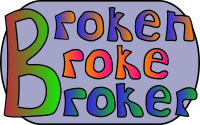
\includegraphics[width=0.6\textwidth]{Bilder/Titelblatt/big_logo.png}
\end{figure}
\todo{Bitte pflegt eure Namen auf dieser Seite!}
\newpage
%Inhaltsverzeichnis
\renewcommand{\contentsname}{Inhaltsverzeichnis}
\tableofcontents
\newpage
%Ab hier bitte neuen Stuff von euch pflegen!

\section{Überblick}
%In diesem Abschnitt bitte nur einen Überblick über die Ziele dieses Projekts geben!

In diesem Abschnitt werden die Gedanken, welche bei der Entstehung der App getätigt wurden, erläutert. Man findet hier die Erläuterungen um die einzelnen Gedankengänge beim Entstehen der App nach zu vollziehen und das Gesamprodukt richtig einordnen zu können.

\subsection{Wodrum geht es in der App Broken Broke Broker}
In der App Broken Broke Broker geht es um die Simulation einer Börsenumgebung in der, der Nutzer einzelne Wertpapiere, Währungen oder Kryptowährungen kaufen kann. Auf dem Smartphone wird ein Spiel begonnen indem es um den Handel mit Wertpapieren geht. Die Kursdaten werden dabei aus dem Web gezogen. Die App soll in Java geschrieben werden und die einzelnen Anwendungen sollen möglichst intuitiv von dem Benutzer zu bedienen sein. Die Menüführung soll klar strukturiert und in einem Stil sein, der es möglich macht sich voll auf den Handel mit Devisen und Wertpapieren zu konzentrieren.

\subsubsection{Anforderungen}
Folgende Features sollen mir der oben gewählten Technologie umgesetzt werden:

\begin{enumerate}
\item 

\item

\item

\item
\end{enumerate}

\subsection{Motivation}
%In diesem Abschnitt bitte nur beschreiben, wie die Zielvorstellung aussieht.
Die Motivation für uns bei diesem Code Camp die App in Java zu schreiben liegt vor allem darin sich als Team einer unbekannten Herausforderung zu stellen. Eine Herausforderung an deren Ende ein Programm steht, welches Spaß beim Spielen macht und einen Einblick in die Welt des Finanzmarktes gibt. Die App heißt Broken Broke Borker um die Tatsache zu verdeutlichen, dass es um 

\subsection{Herangehensweise}
%Wir die einzelnen Ziele erreicht werden sollten werden wir in diesem Abschnitt hinterlegen!

\section{Funktionalität der Application}
%Beschreiben der einzelnen GUI Oberflächen und deren Funktion. 
%Bitte selbstständig die einzlenen Abschnitte mit den Screens ergänzen!


\subsection{Technische Details}

\subsection{Verwendete Programmierbibeotheren}

\subsection{Navigationsshma zwischen den Bildschirmen}

\subsection{Liste aller Klassen und deren Methoden mit Funktion}

\section{Klassendiagramm}

\subsection{Anbindung an das Datenmodell der API}

\subsection{Darstellung des Datenmodells als UML}

\subsection{Darstellung aller Views und deren Controller als UML}

\section{Überlick über die Umsetzung}
%Hier ist wichtig zu schreiben, was wir meinen Gut gemacht ist und wie dies mit den App zielen conquentiert.

\section{Fazit}
%Hier ist wichtig, dass wir es schaffen können zu zeigen, ob wir mit den erreichten Zielen zufrieden sind.





\end{document}